\chapter{Anexos}
\label{ch:anexos}

\section{Ideas recopiladas de la sesión de \textit{Design Thinking}}
\label{sec:designthinking}
\begin{itemize}
    \item \textbf{Aspectos positivos}
    \begin{itemize}
        \item Pensar y actuar, comprometerme.
        \item ¡Armarse de valor! Empezar y luego ir mejorando aspectos, uno por uno.
        \item Sienten que la universidad no fomenta el trabajo en equipo cuando es algo que las empresas demandan (se ve como algo positivo a aprovechar).
        \item Oigo que las empresas siempre están buscando talentos y gente con ideas para ayudarles a llevarlas a cabo.
        \item Puede dar difusión a una buena idea.
        \item El TFG de mi carrera es muy aburrido (visto como oportunidad).
        \item Veo posibilidades de mejorar la realidad física a través de la realidad virtual. Pensar.
        \item Es una oportunidad de crear proyectos interesantes y experiencias.
        \item Proponer herramientas online y virtuales y generar documentación.
        \item Múltiples posibilidades. Inquietud.
        \item Trabajar duro para llegar a la cohesión. Investigar acerca de todo, el máximo posible. Afrontar el proyecto sin temor al fracaso.
        \item Frustración por no desarrollar una idea propia.
        \item Apostar por ideas innovadoras de TFG. Buscar ideas/productos interesantes para motivar.
        \item Veo un gran distanciamiento entre los distintos campus y no saben lo que pasa entre unos y otros.
    \end{itemize}
    \item \textbf{Ideas}
    \begin{itemize}
        \item Identidad visual.
        \item Comunicación.
        \item Plataforma web.
        \item Jornadas de estudiantes como forma de conocer sus necesidades e incertidumbres.
        \item Fomentar espacios virtuales para comunicación, reuniones y conocimiento.
        \item Fomentar espacios físicos de debate y trabajo (ámbito lúdico, forma de llegar a la sociedad).
    \end{itemize}
    \item \textbf{Objetivos}
    \begin{itemize}
        \item Mapa geográfico de proyectos que permitan acceder al proyecto.
        \item Proyectos conectados entre sí, por tipo.
        \item Hay que crear grupos muy comprometidos y concienciados.
        \item Dificultades, reuniones
        \item Posibilidad de llegar a todos.
        \item Exposición en público.
        \item Crear congresos y seminarios sobre el proyecto interdisciplinar.
        \item Síntesis de ideas para transformarlas en contenido a exponer en redes y otros medios y así dar repercusión al proyecto.
    \end{itemize}
    \item \textbf{Limitaciones}
    \begin{itemize}
        \item No se conoce. Dudas acerca de la viabilidad. No lo entienden. Les atrae como para crear una empresa.
        \item Cómo dar más difusión a los trabajos TFG.
        \item Huimos del tema por miedo a suspender. Vamos a lo fácil para sacar la carrera y no nos complicamos.
        \item Oigo que la gente tiene buenas ideas que le gustaría desarrollar, pero les falta gente que sepa de ciertas cosas.
        \item Cuesta trabajo encontrar tiempo para dedicárselo.
        \item No hay espacios para trabajar en grupo. No hay espacio ni tiempo suficiente para trabajar.
        \item Es un mayor esfuerzo de lo que parece habitual.
        \item No hay tiempo y faltan espacios.
        \item Grandes ideas, propuestas interesantes. Pero hay limitaciones de tiempo y material.
        \item Inseguridad. Ilusión por realizar algo innovador. Falta de un anteproyecto que una las diferentes ramas.
        \item Hay que conformarse con el TFG establecido.
        \item Oigo a la gente quejarse de que trabajar en equipo a veces no sale bien.
        \item No hay tiempo para reuniones y organizar.
        \item Exceso de trámites para realizar un TFG.
        \item Piensan que trabajar en equipo es un engorro y que siempre sale mal.
        \item No existen herramientas para hacer diferentes TFG.
        \item Falta de ayuda por parte de la universidad y el ayuntamiento.
        \item Como ven que es difícil trabajar en equipo, lo que hacen es conformarse con un proyecto más simple que les gusta menos.
        \item Con desesperación, con esperanza, con oportunidades.
        \item Necesidad de implicación (nosotros mismos, menos integrantes). Necesidad de sintetizar las ideas. Si una persona no conoce el proyecto, o quiere participar, una idea clara.
        \item Plazos y forma de organización a veces muy rígida.
        \item Veo que la gente no está motivada a trabajar en equipo y prefieren trabajar solos.
        \item Incertidumbre, amparo, curiosidad.
        \item Inestabilidad, falta de conexión.
    \end{itemize}
\end{itemize}

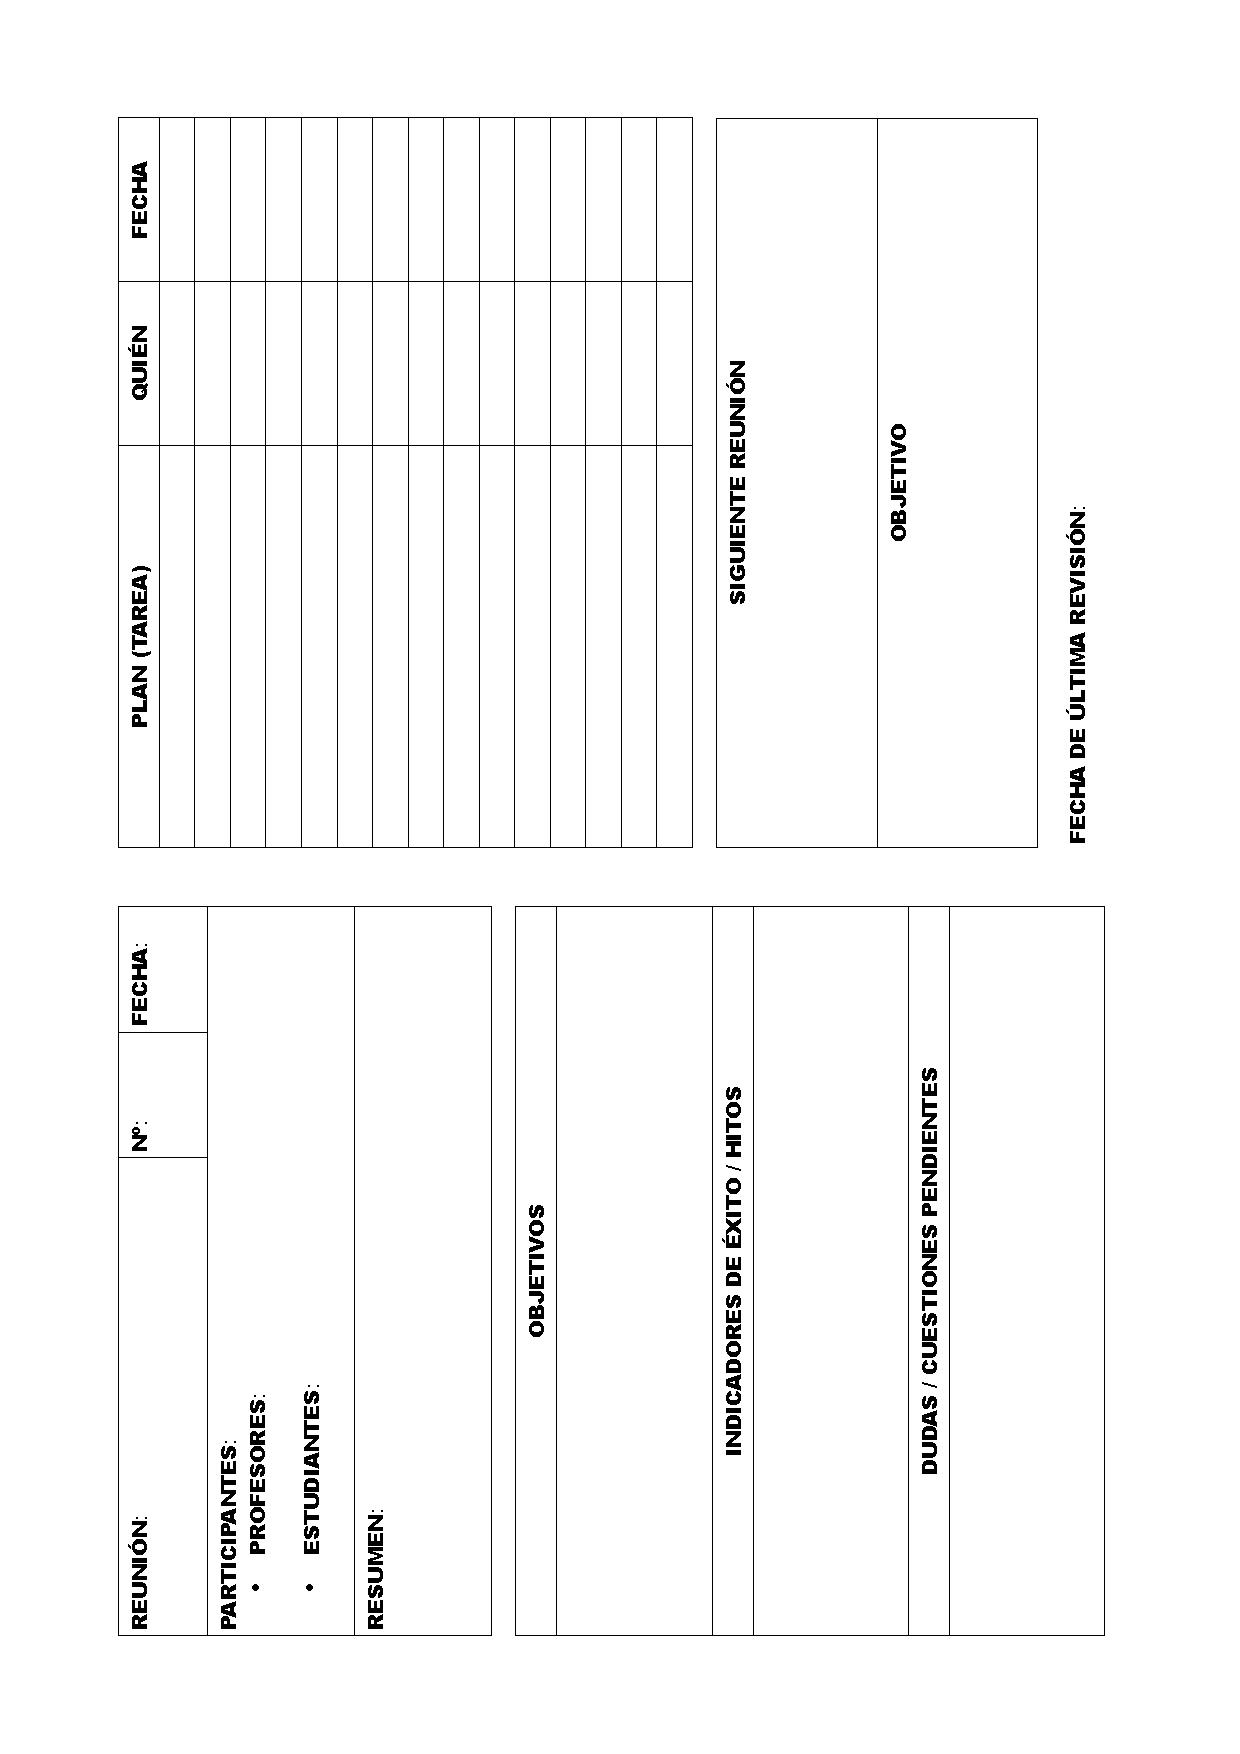
\includepdf[pages=1-]{meetings/template.pdf}

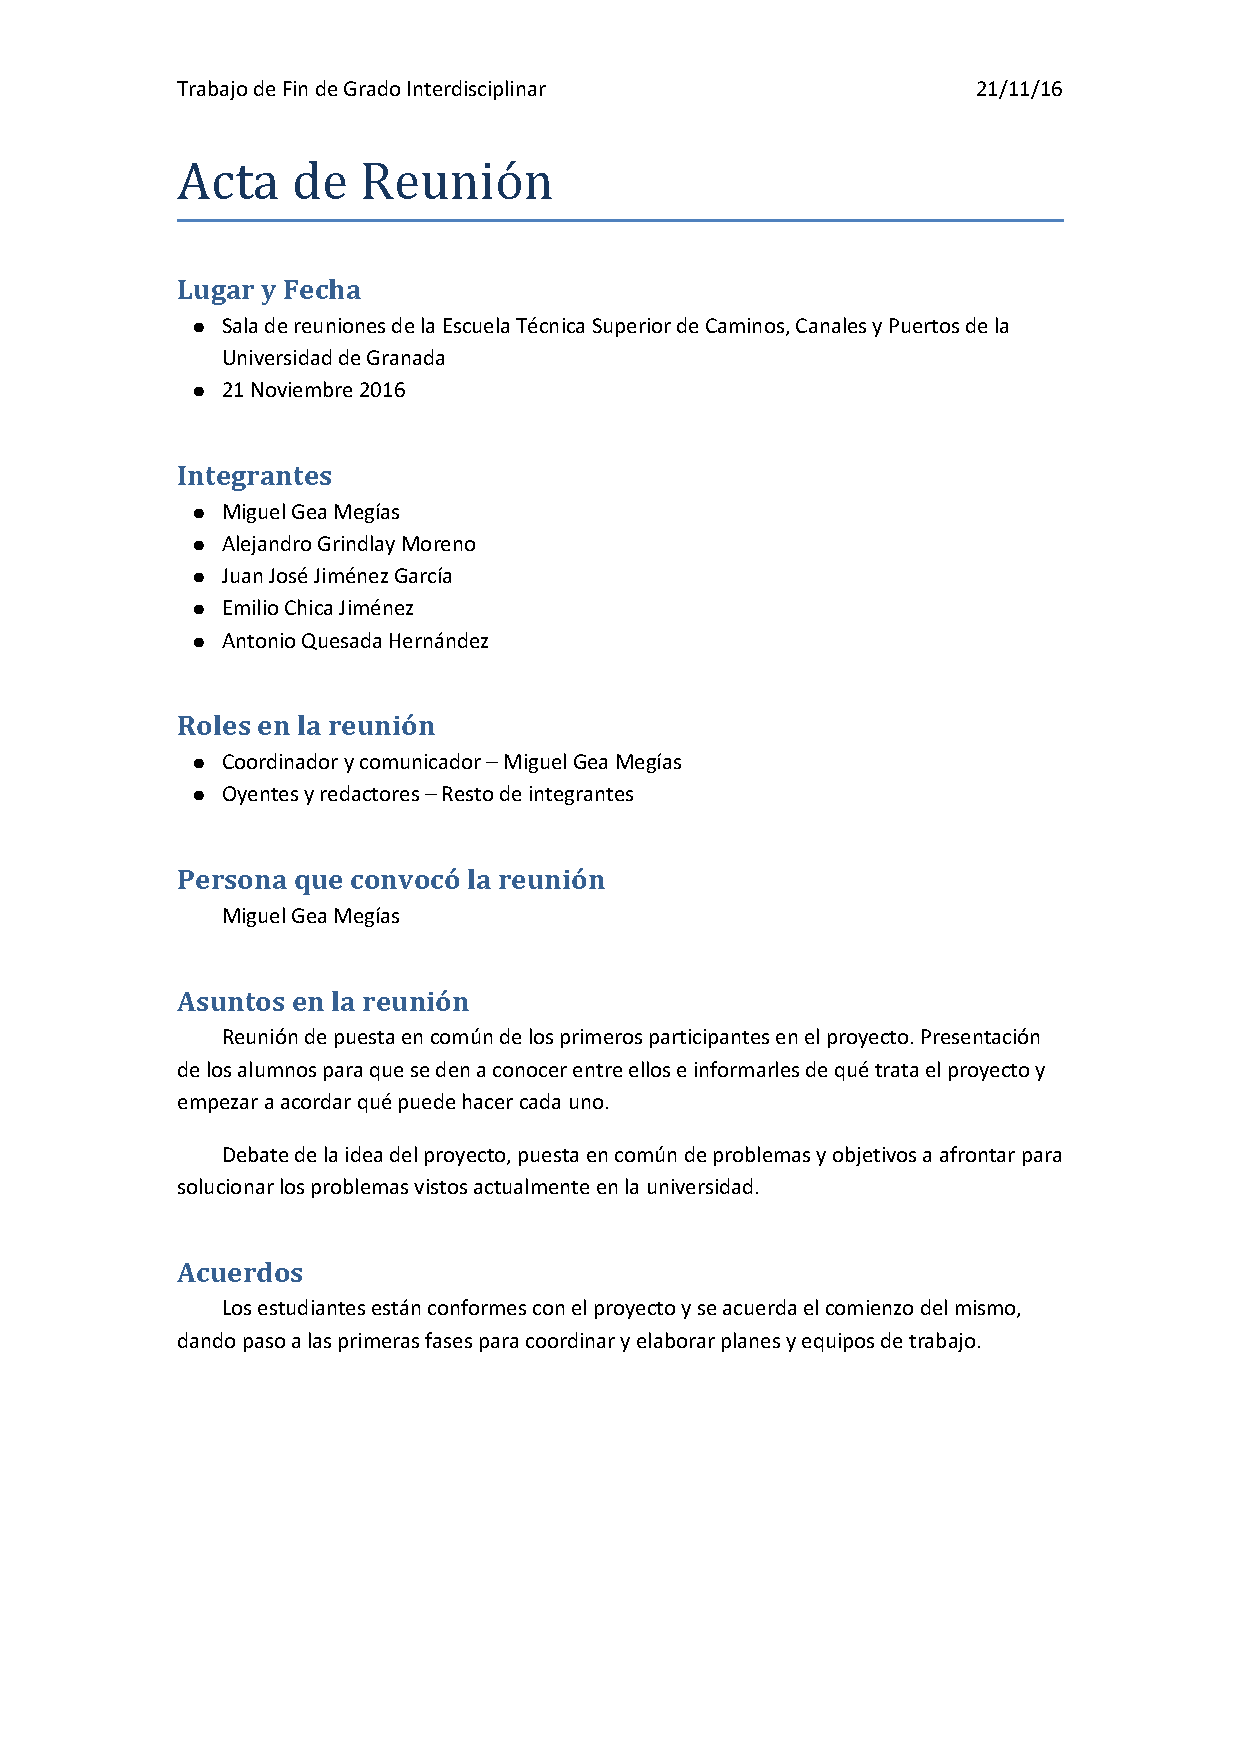
\includepdf[pages=1-]{meetings/01.pdf}
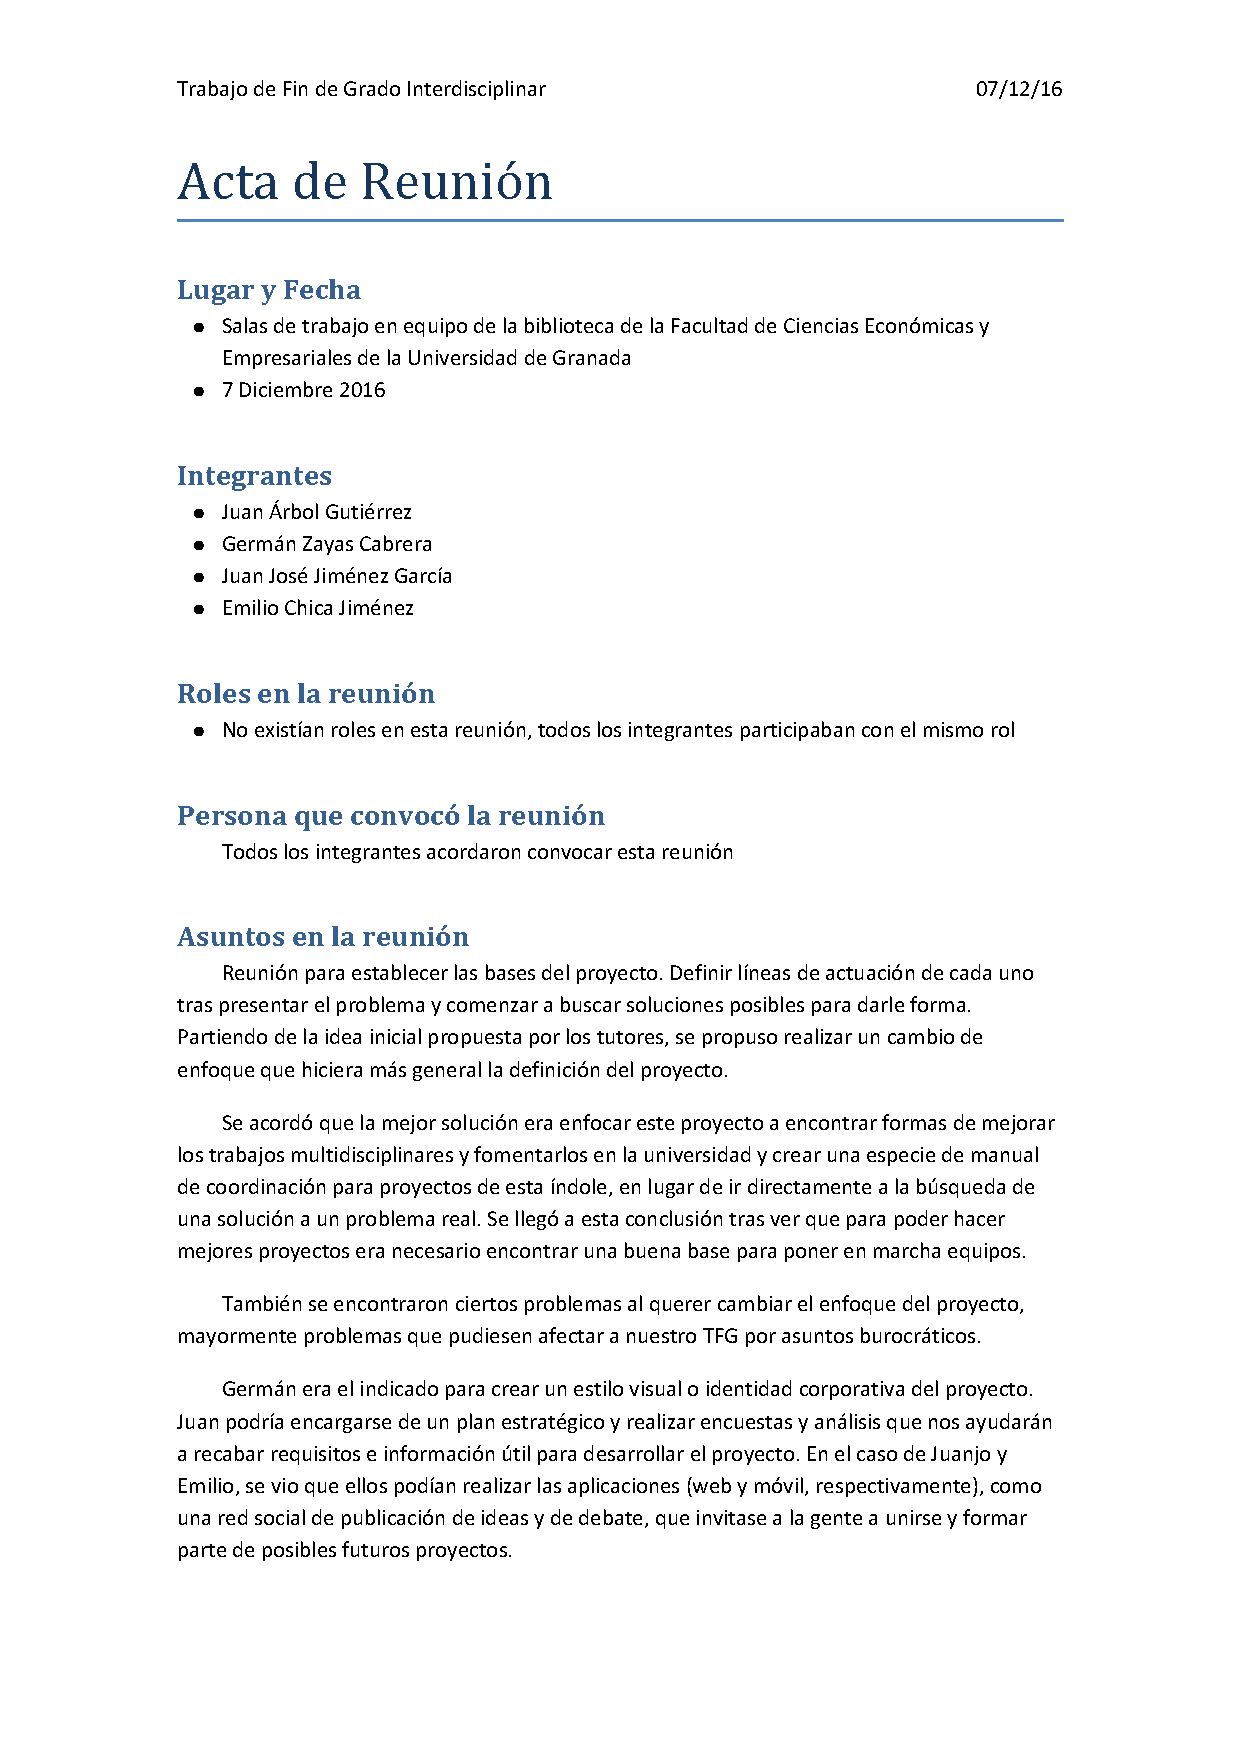
\includepdf[pages=1-]{meetings/02.pdf}
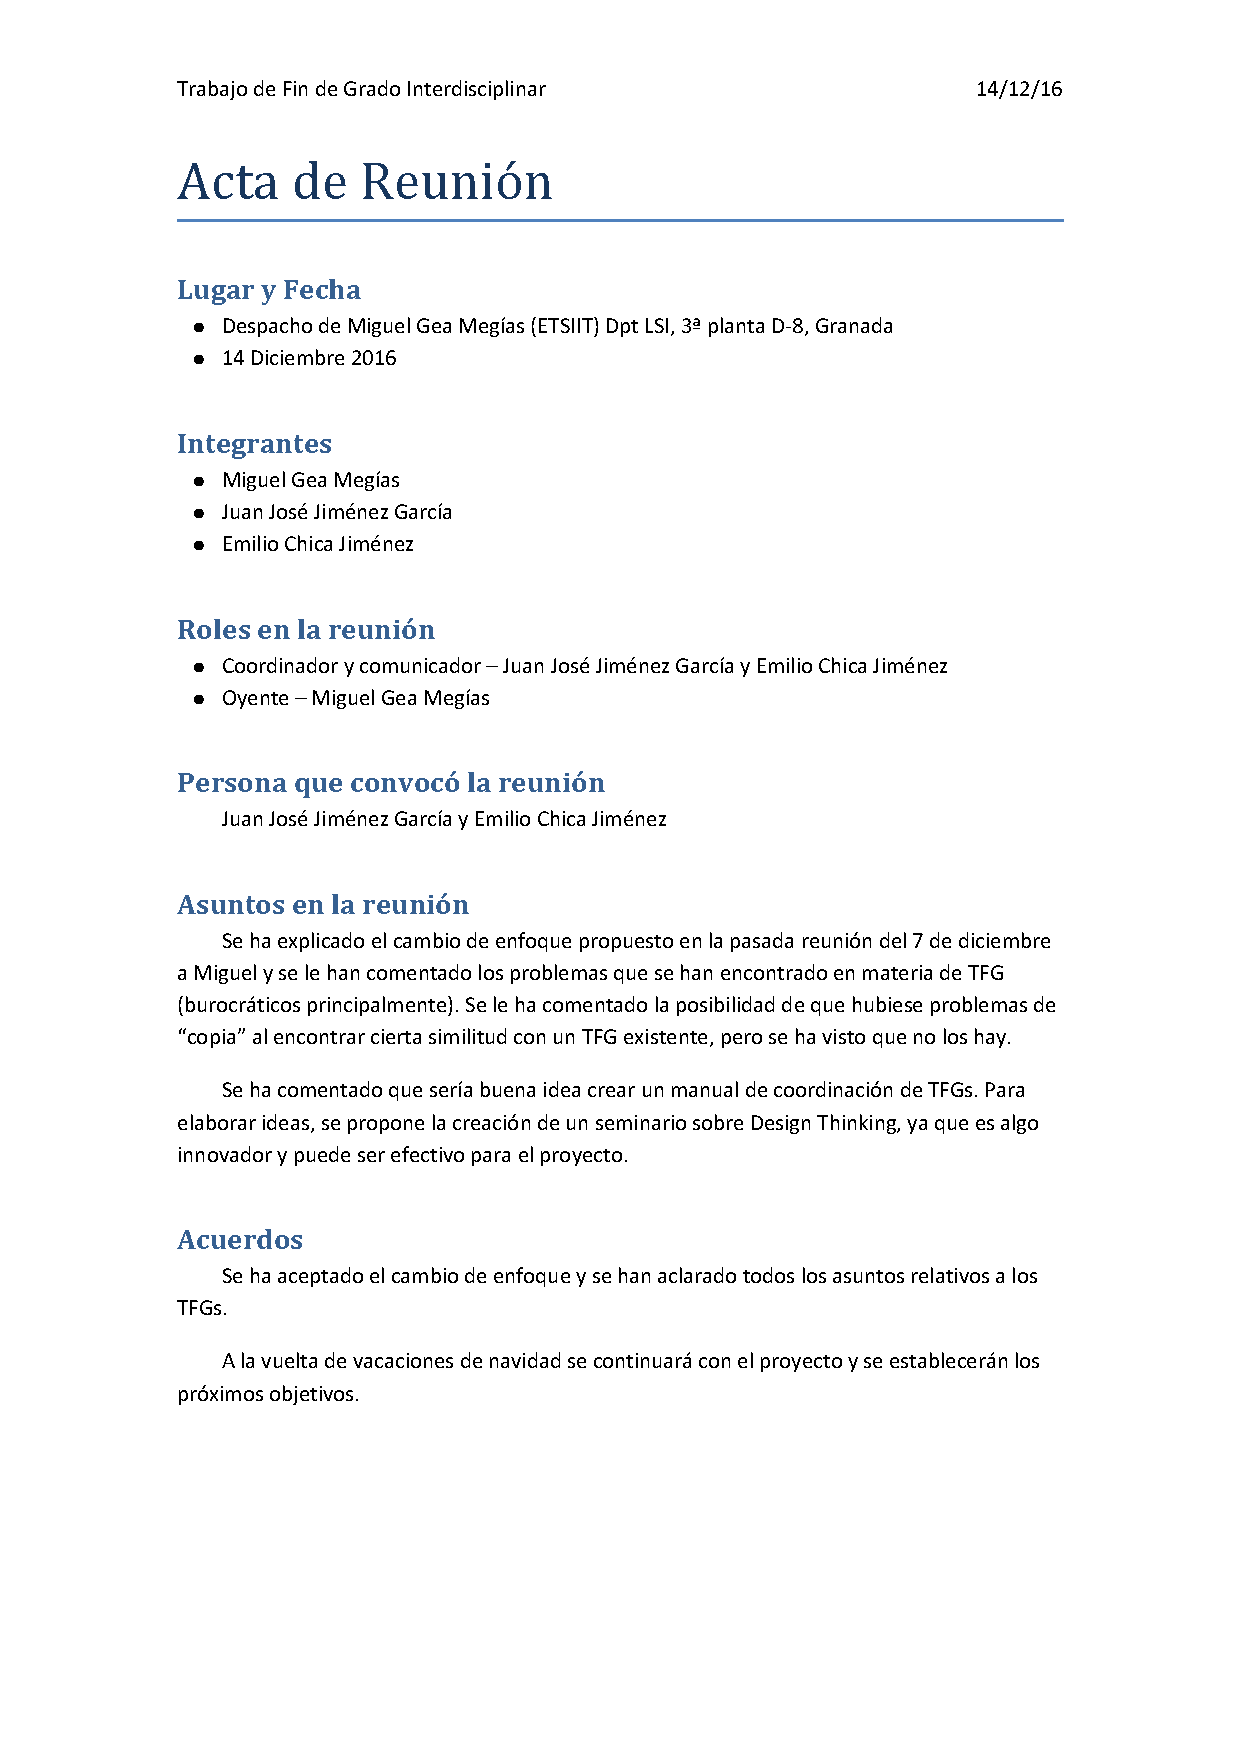
\includepdf[pages=1-]{meetings/03.pdf}
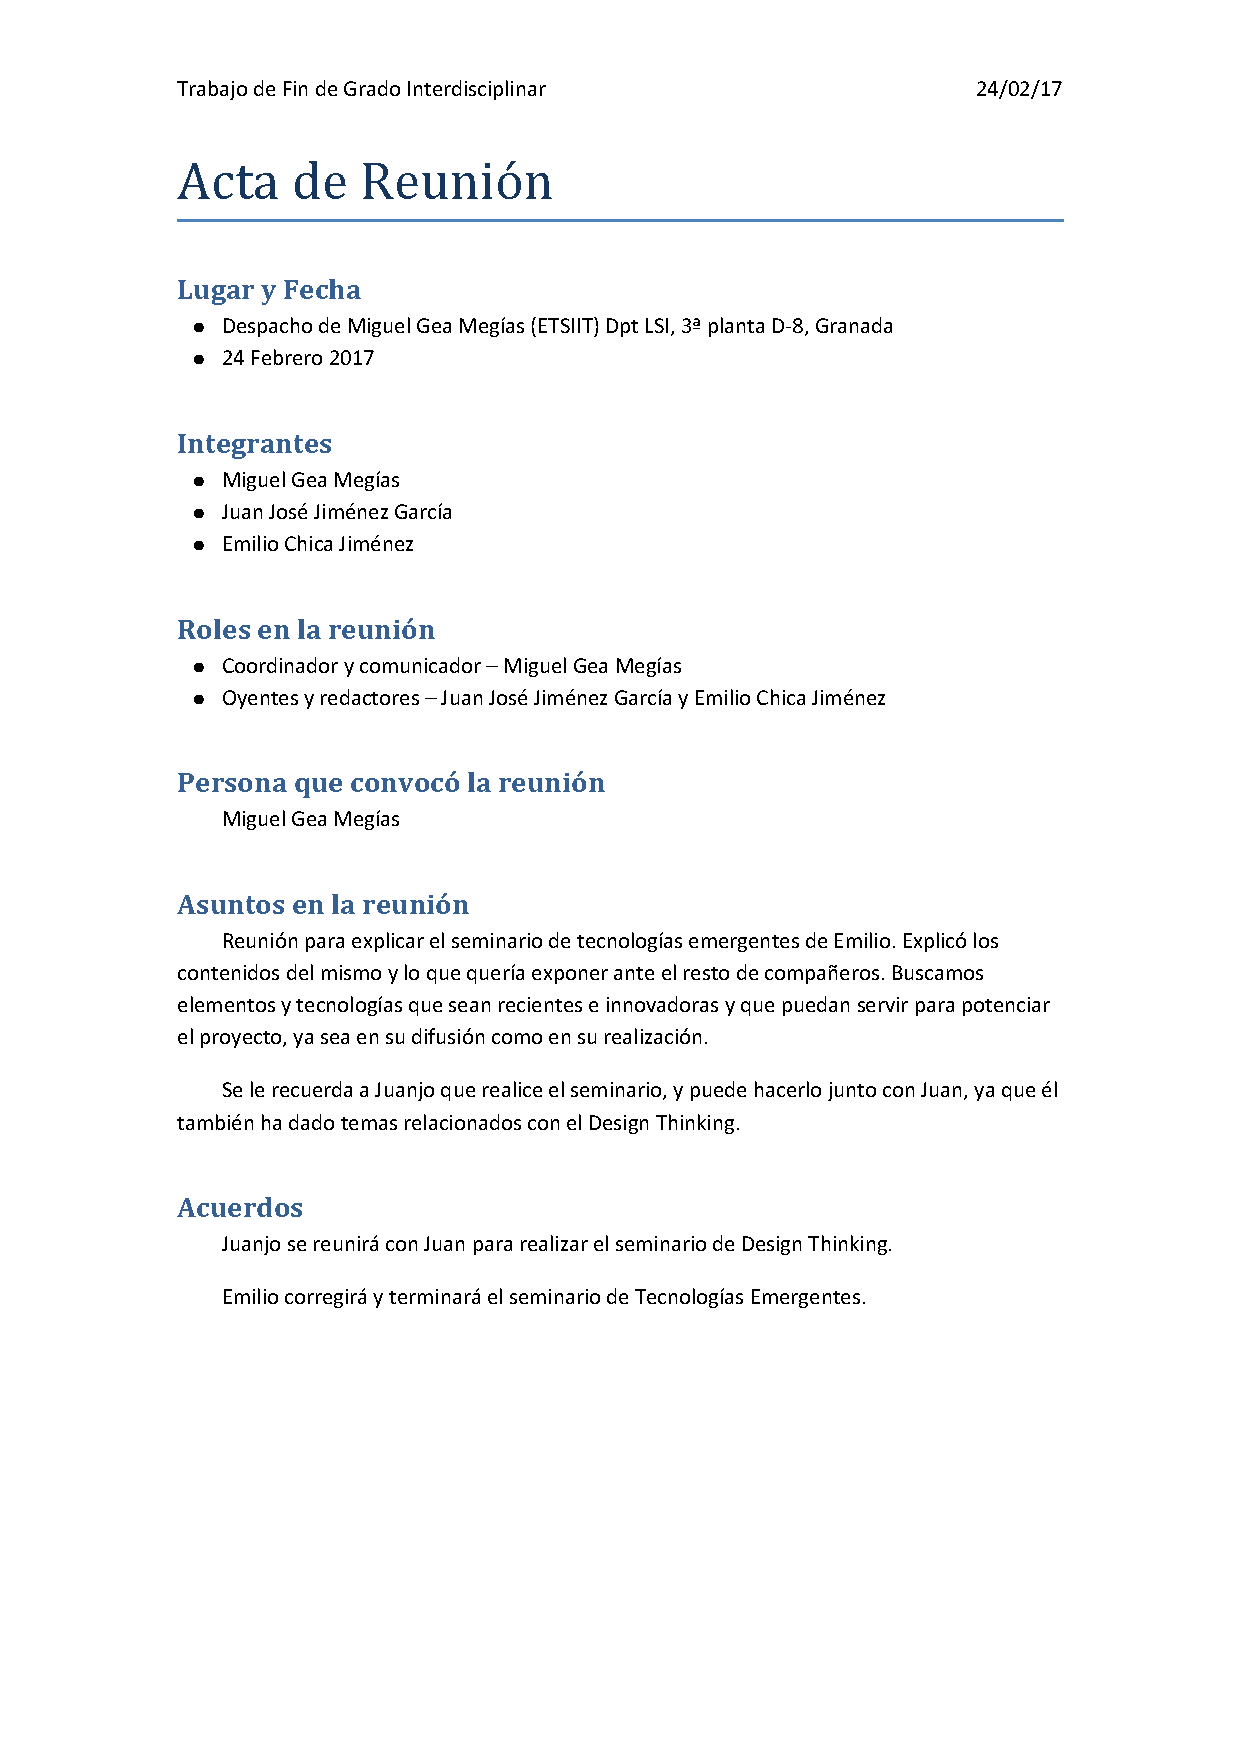
\includepdf[pages=1-]{meetings/04.pdf}
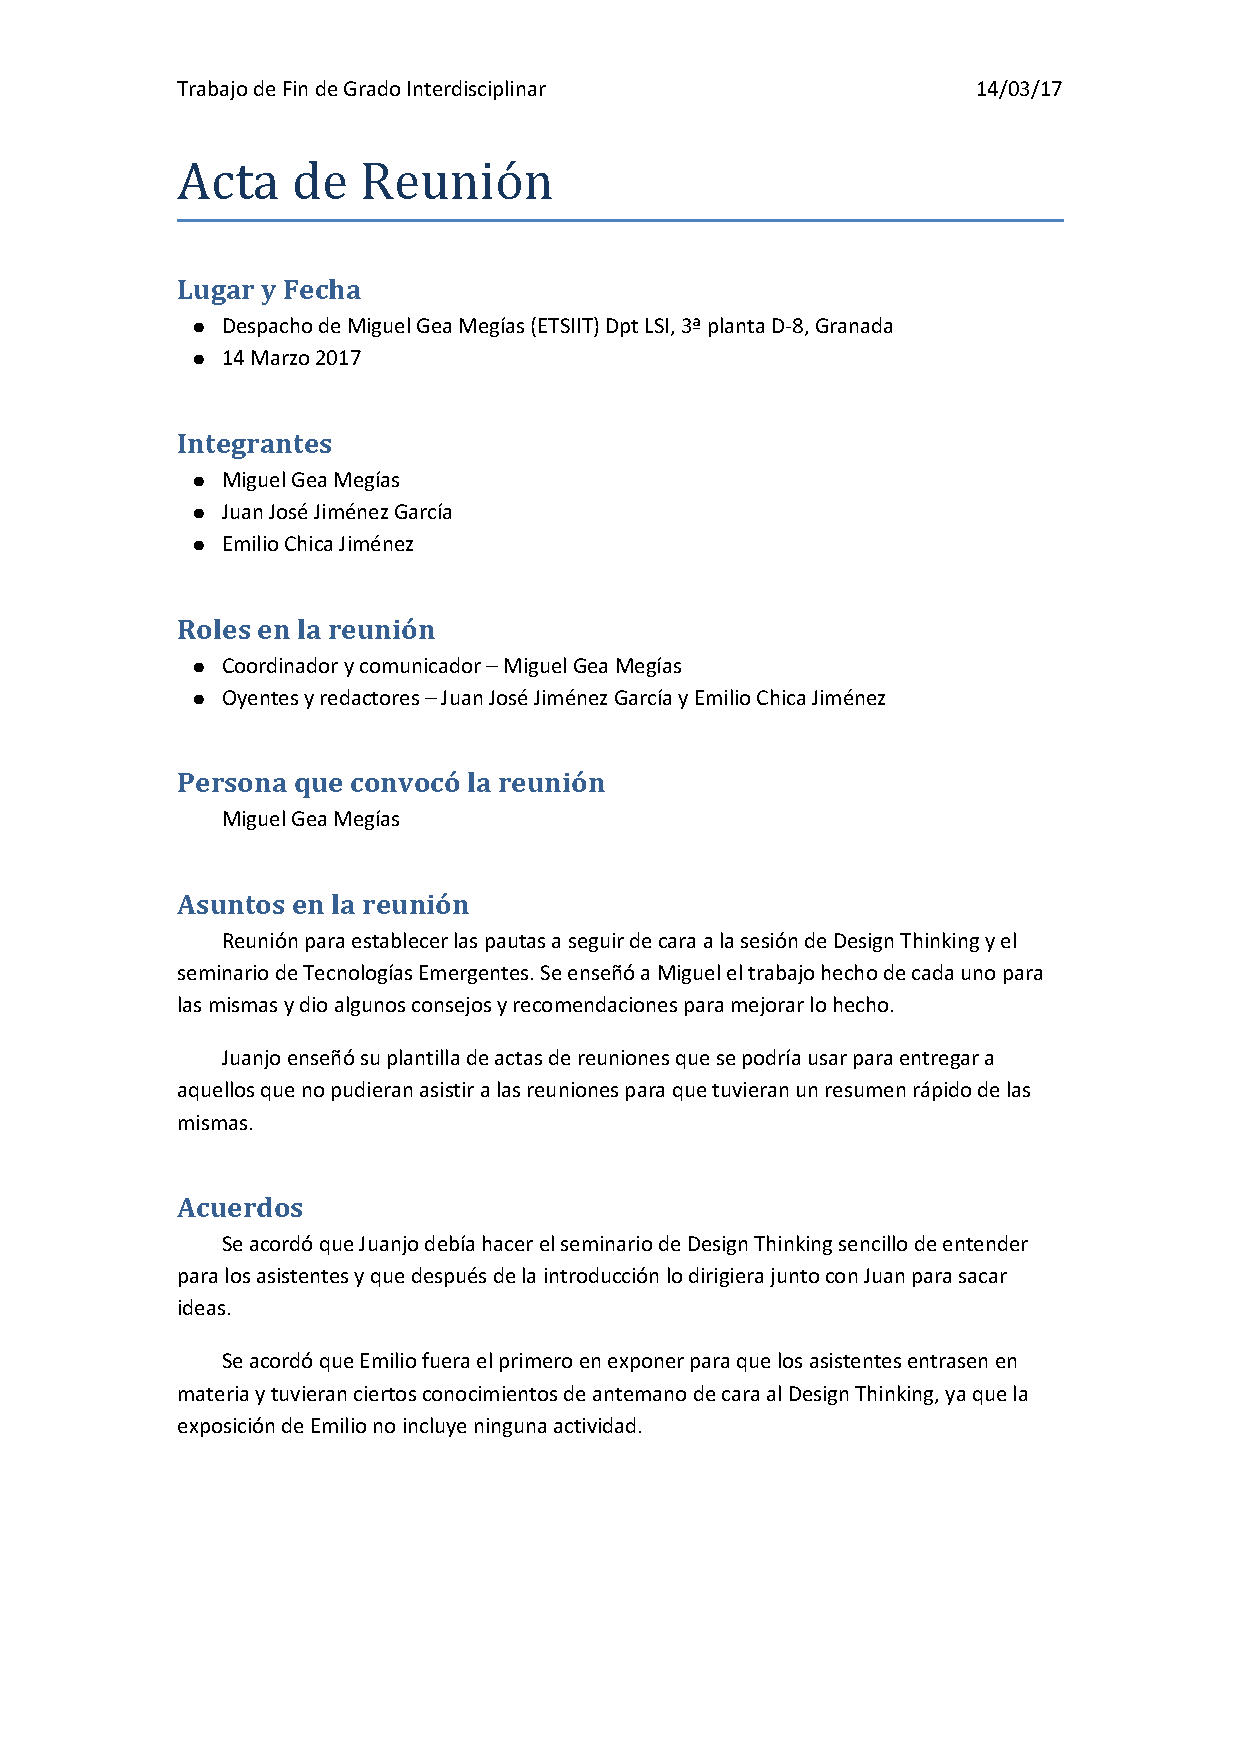
\includepdf[pages=1-]{meetings/05.pdf}
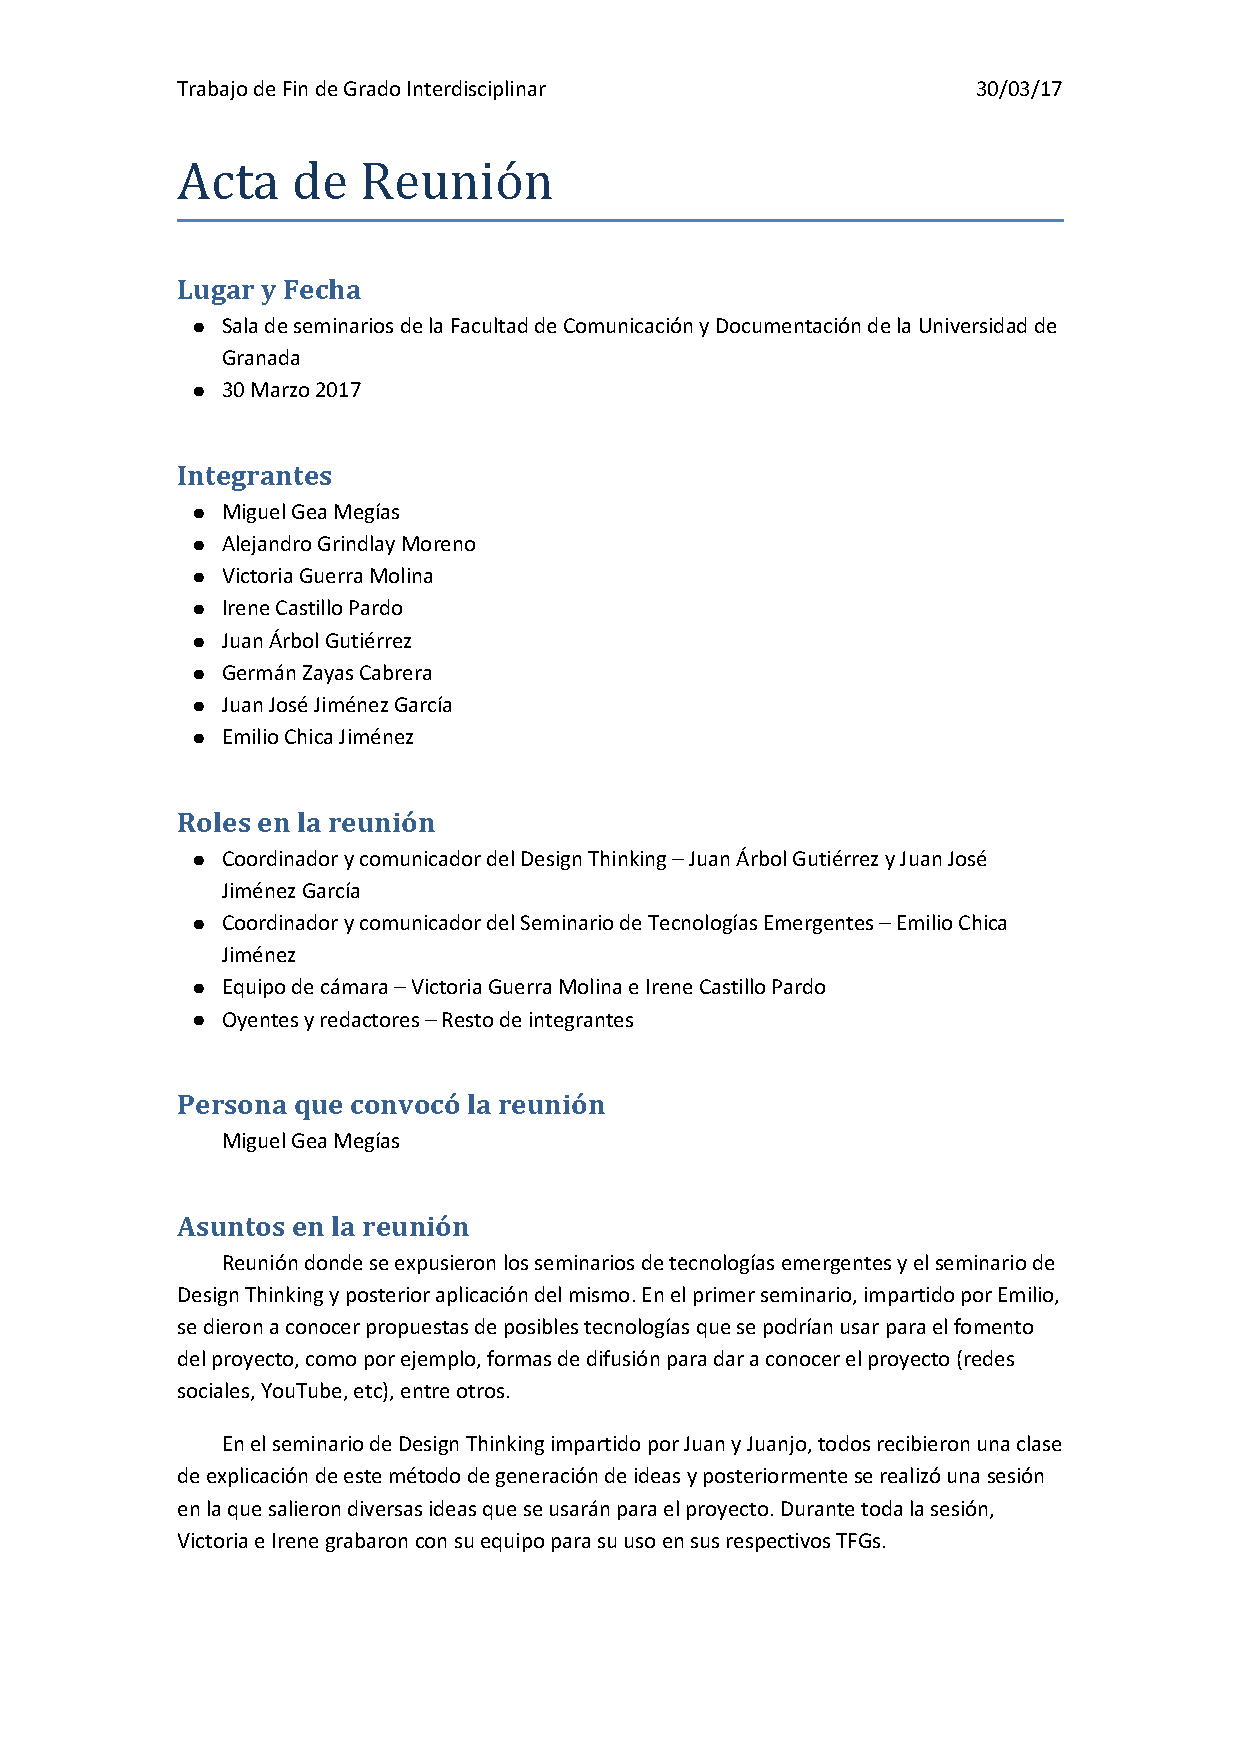
\includepdf[pages=1-]{meetings/06.pdf}
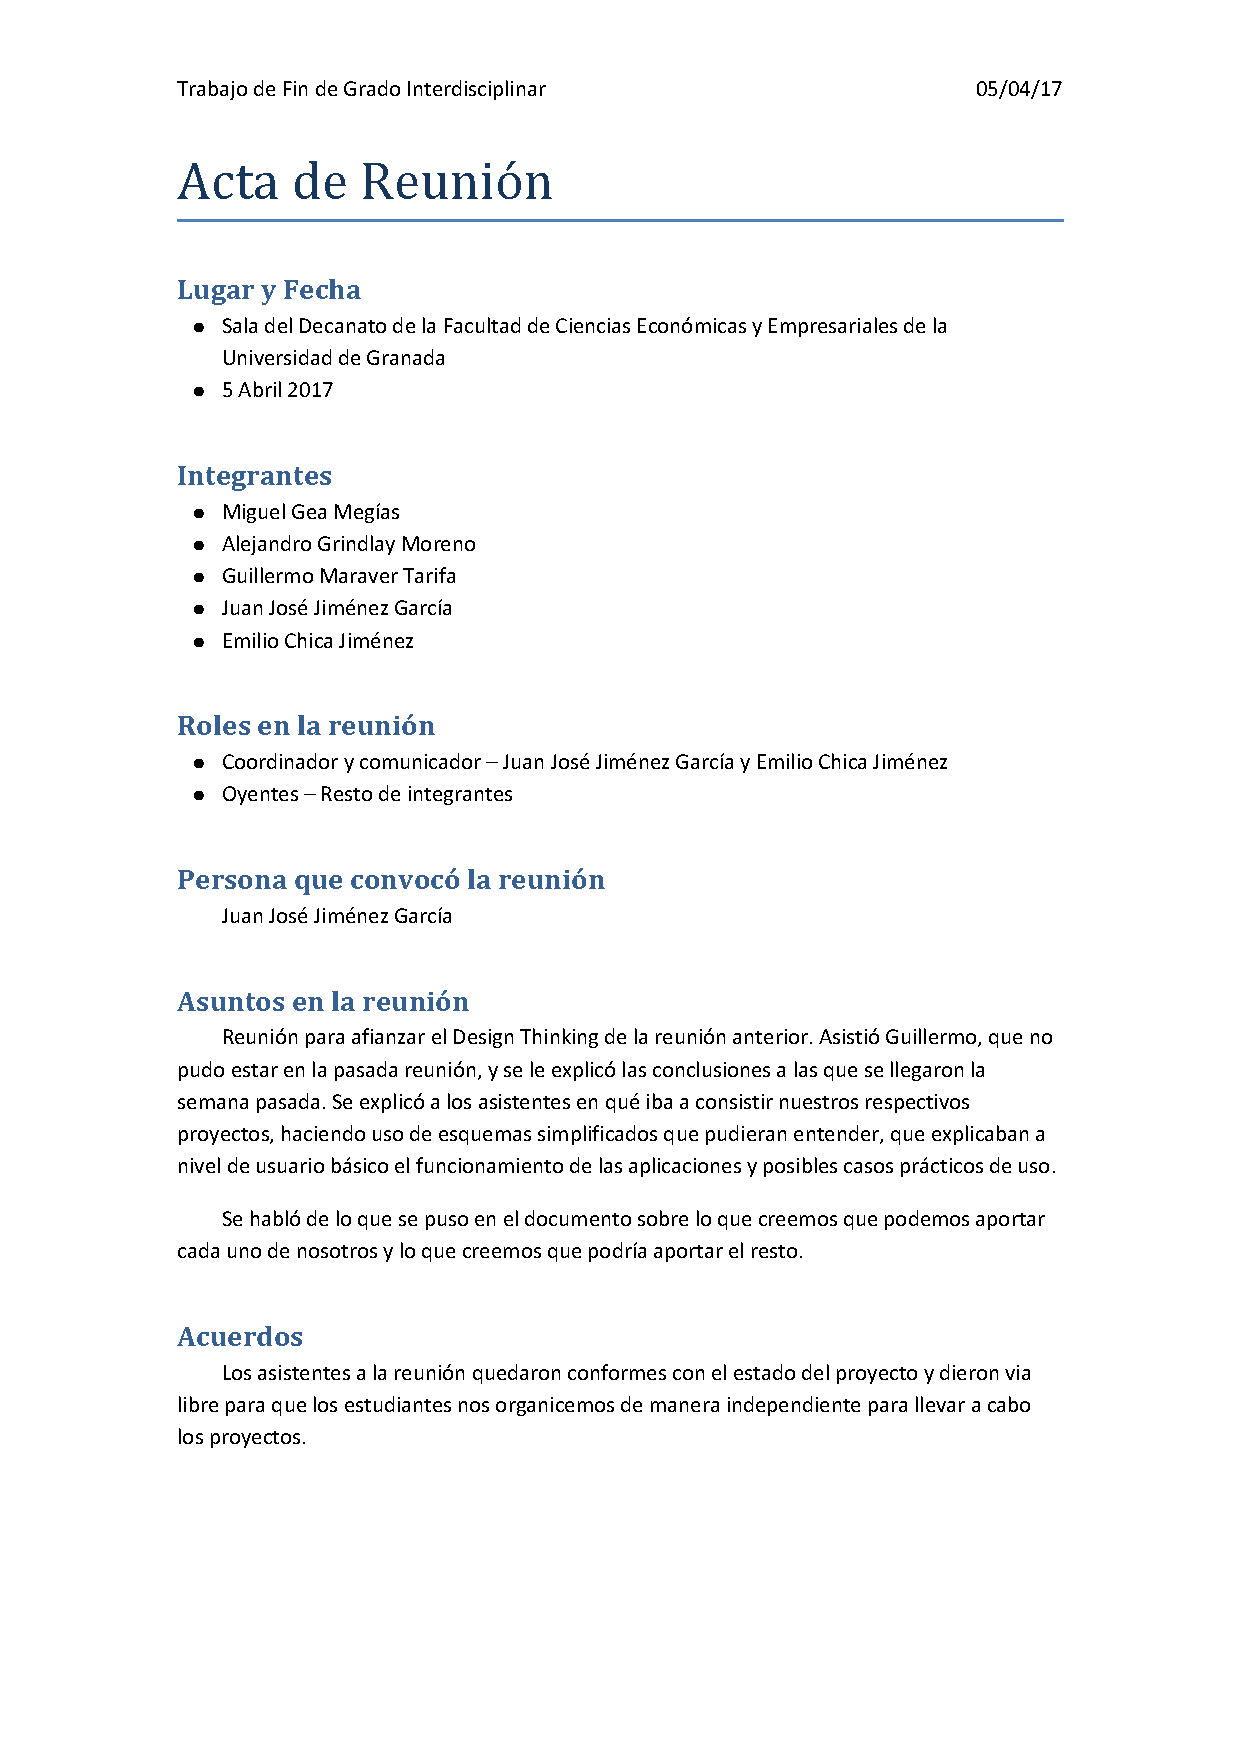
\includepdf[pages=1-]{meetings/07.pdf}
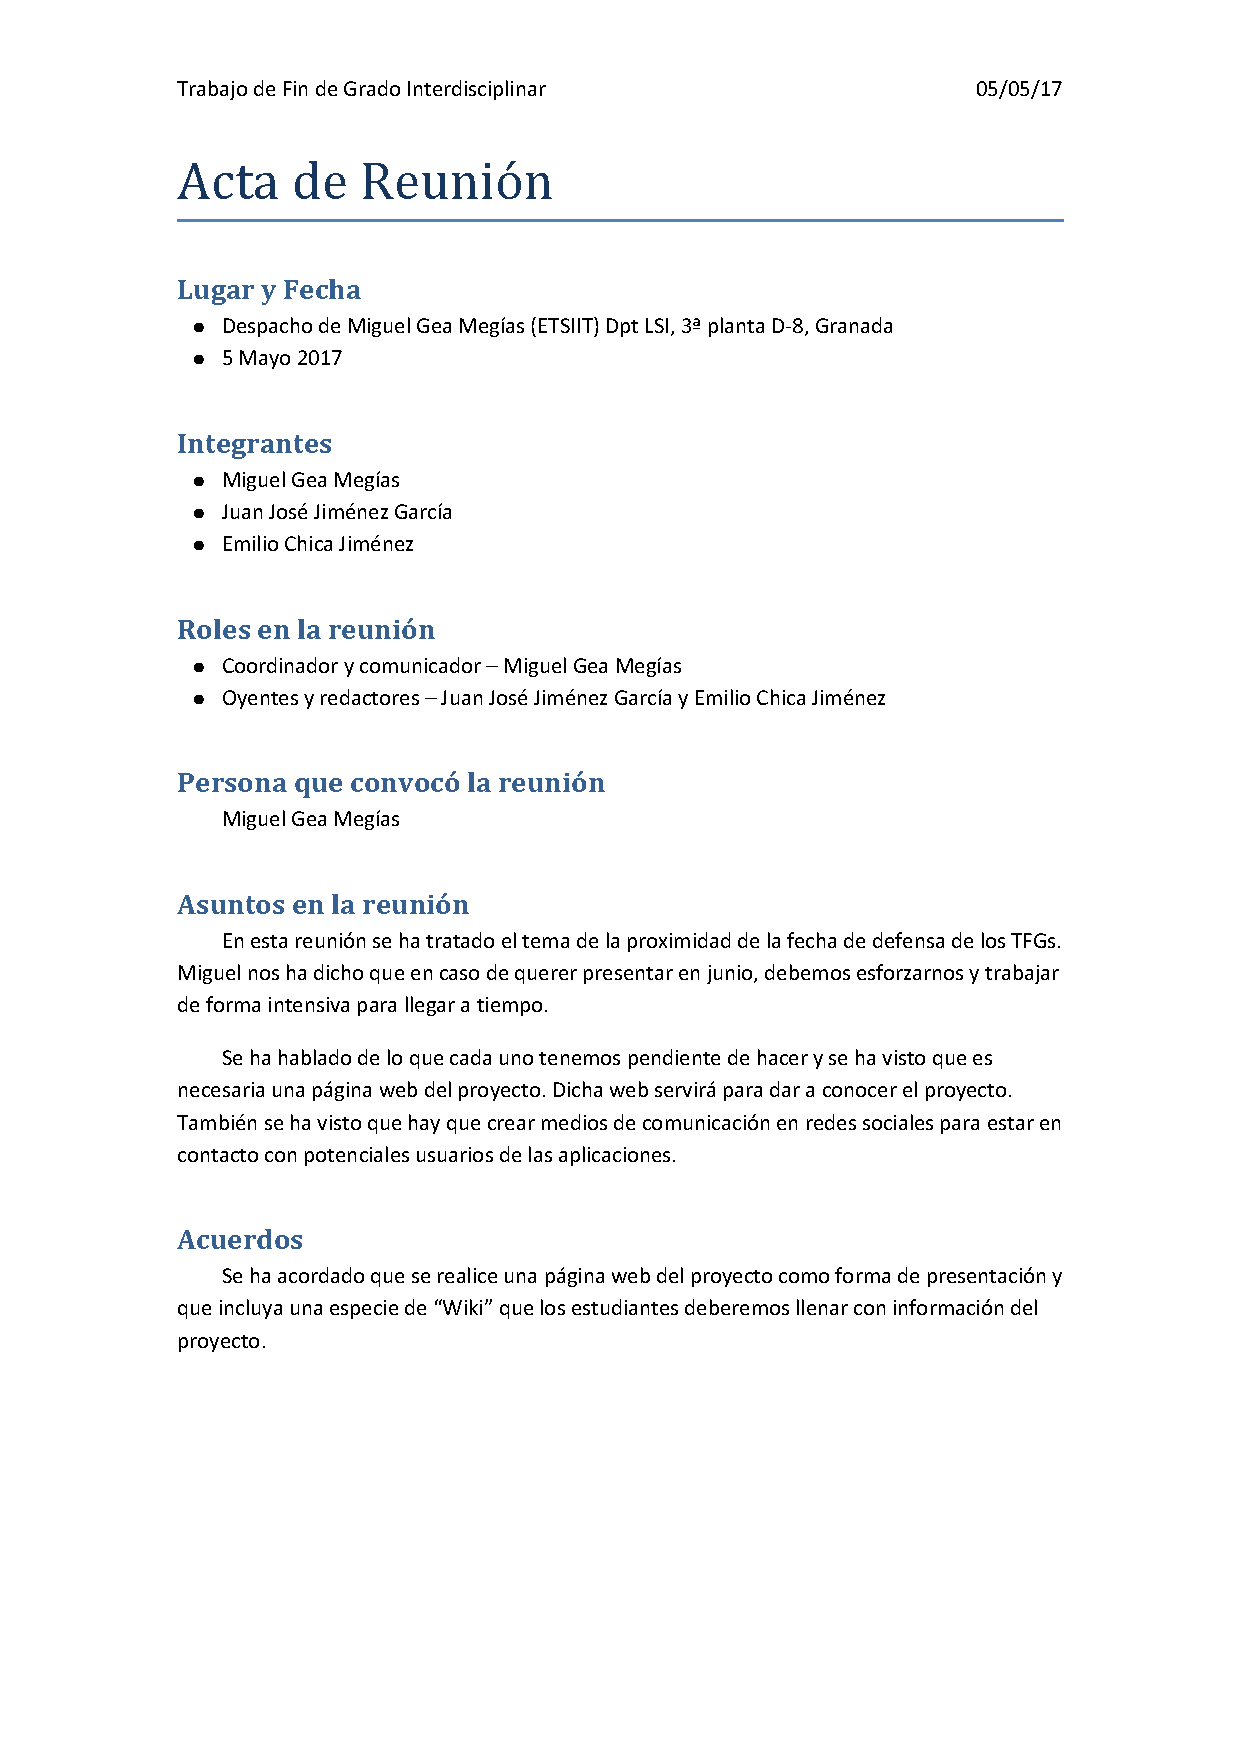
\includepdf[pages=1-]{meetings/08.pdf}
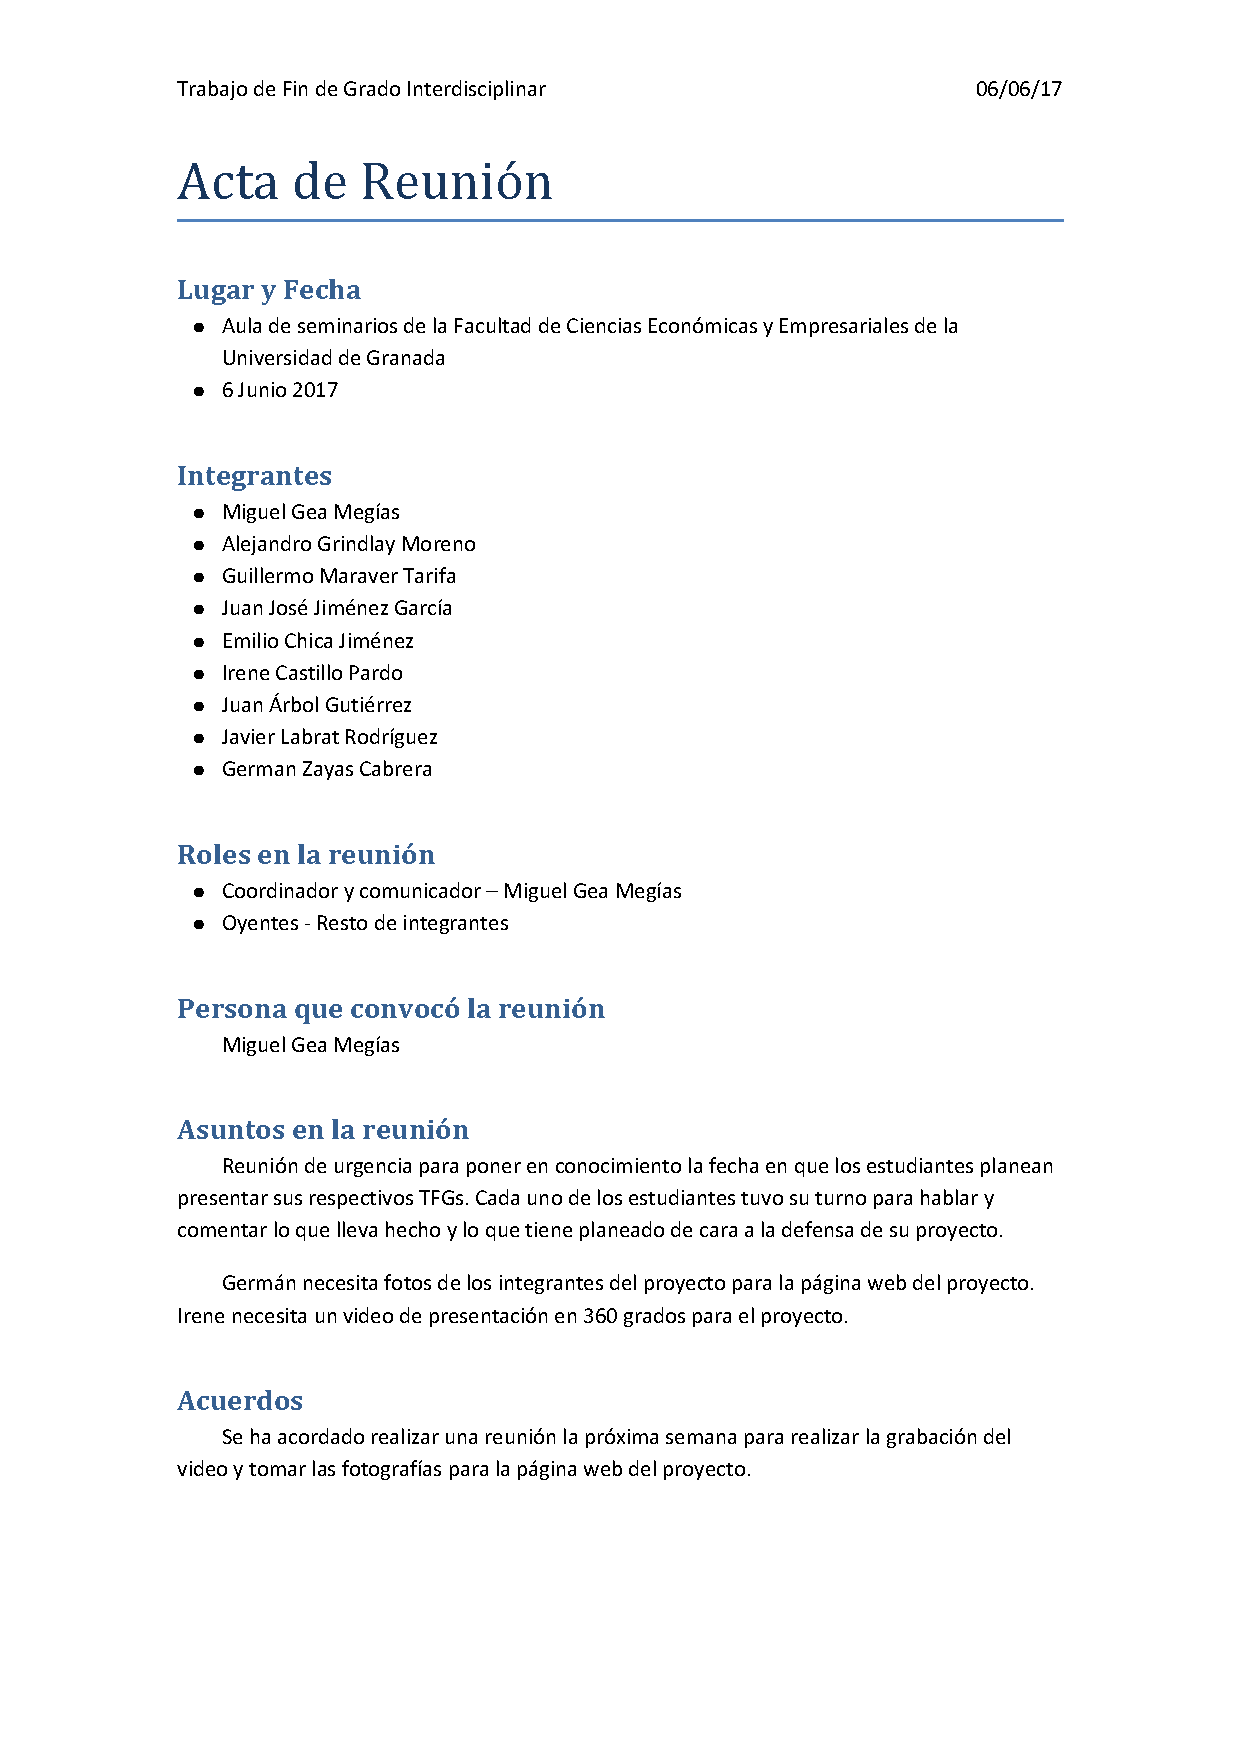
\includepdf[pages=1-]{meetings/09.pdf}
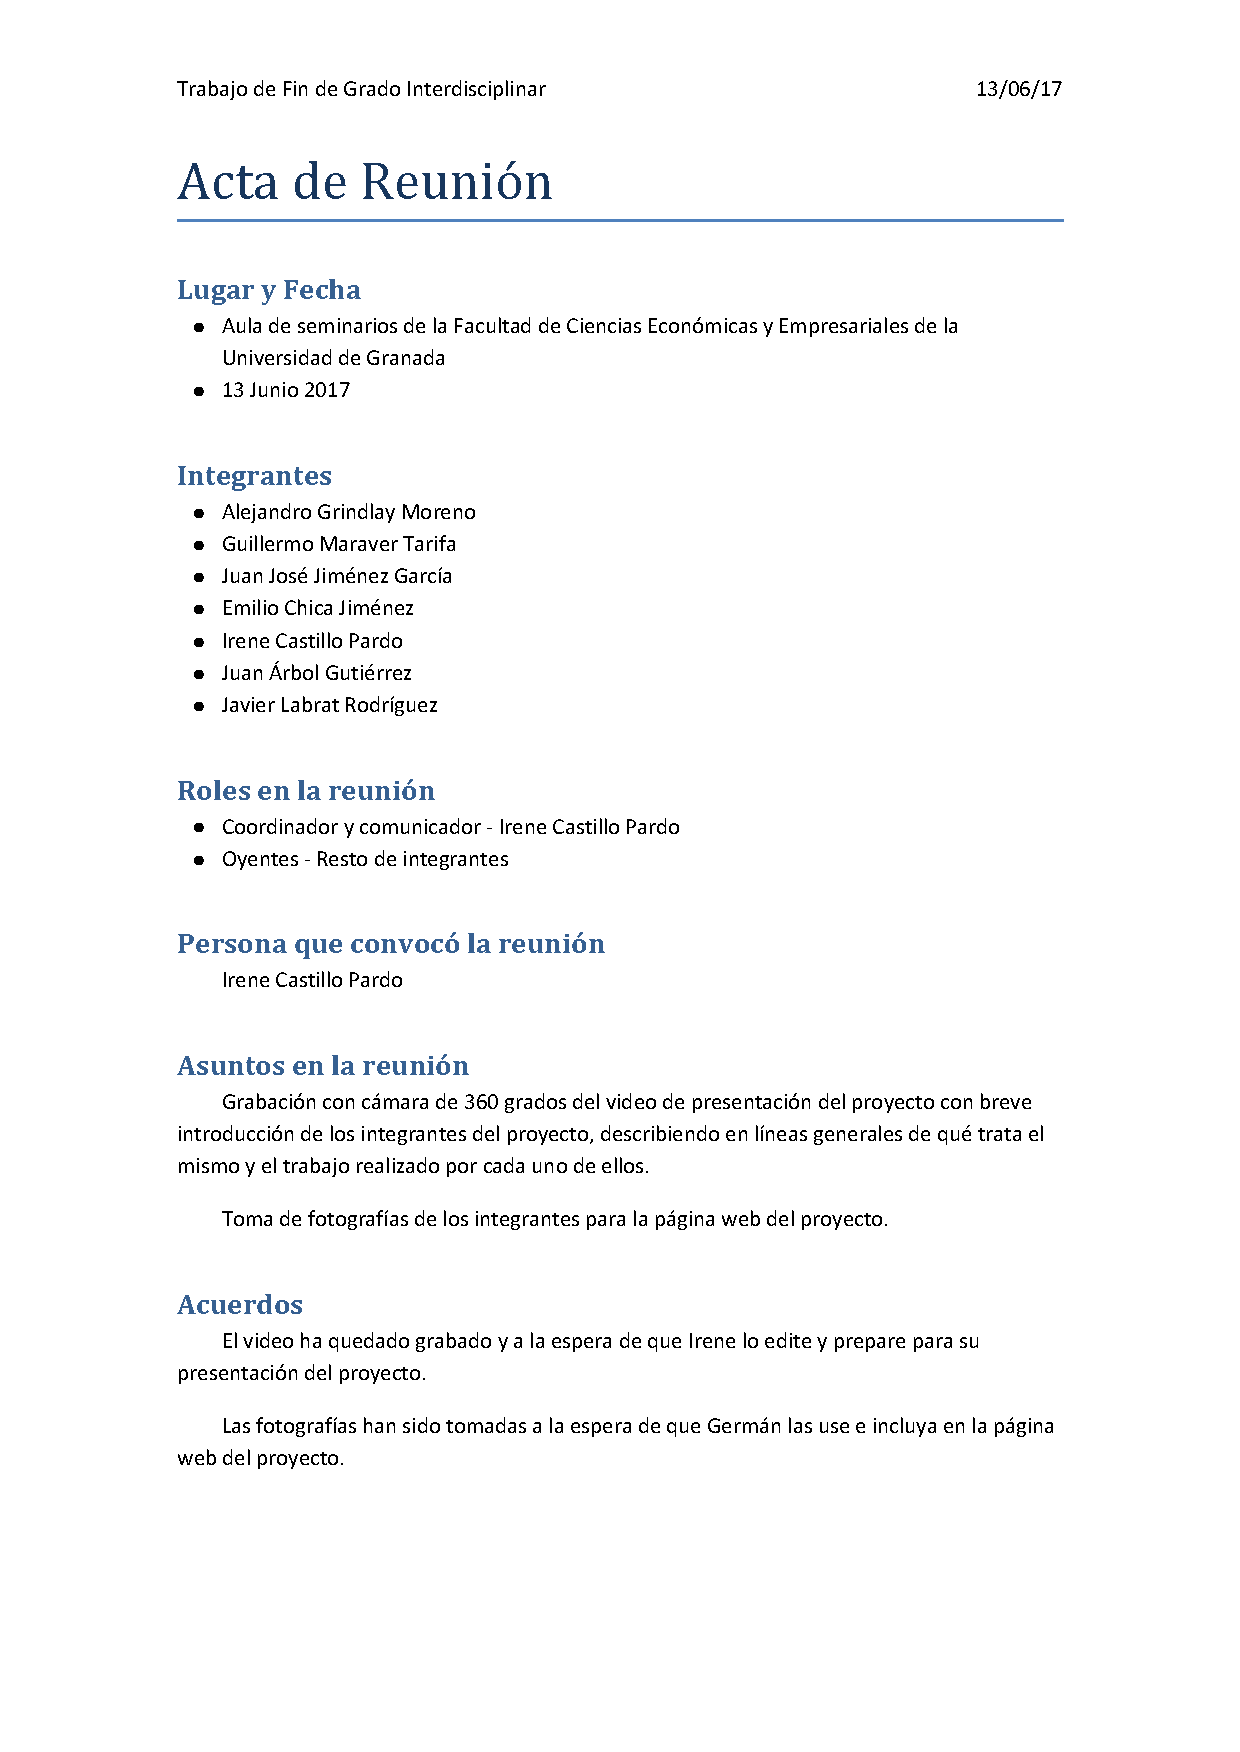
\includepdf[pages=1-]{meetings/10.pdf}
